\section{Graphfärbung}

\textbf{Definition}: Sei $G=(V,E)$ ein Graph, $k\in\N$. 
Eine \textbf{$\boldsymbol{k}$-Färbung} von $G$ ist eine Abbildung $c\colon V\rightarrow \{1,2,\ldots,k\}$, sodass $c(u)\neq c(v)$ für jede Kante $uv\in E$
\begin{itemize}
	\item Kleinstes $k$, für das so eine $k$-Färbung existiert, heißt \textbf{chromatische Zahl $\boldsymbol{\chi(G)}$}
	\item Bei Färbungen nehmen wir Graphen implizit als schlingenfrei an
\end{itemize}
\bigskip
\textbf{Frage}: Was ist die größte chromatische Zahl die ein planarer Graph
annehmen kann, d.h. was ist $\chi_{\text{planar}}\coloneqq\max\{\chi(G)\mid G \text{ planar}\}$?\\

\textbf{Lemma}: $\chi_{\text{planar}}\leq 6$

\begin{wrapfigure}{r}{0.25\textwidth}
	\centering
	\vspace{-55pt}
	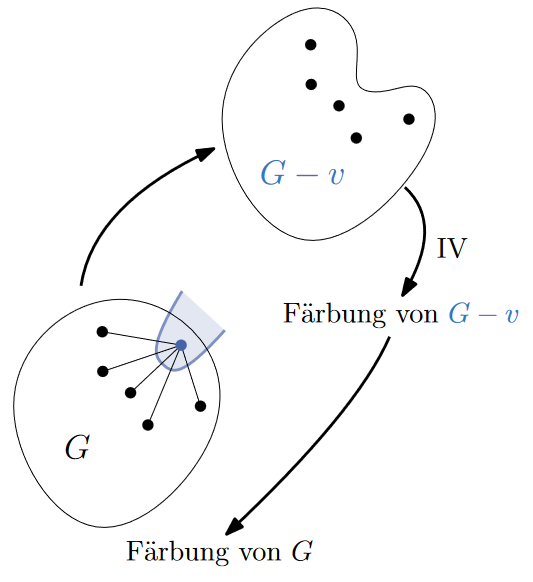
\includegraphics[width=0.3\textwidth]{images/6-f.png}
	\vspace{40pt}
	\vspace{-120pt}
\end{wrapfigure}
\textit{Beweis}: Führe Induktion über $|V|$
\begin{itemize}
	\item I.A.: $|V|\leq 6$: Man erhält eine Färbung, indem jeder Knoten eine eigene Farbe bekommt
	\item I.S.: $|V|> 6$
	\begin{itemize}
		\item Nach Euler-Formel gibt es $v\in V$ mit $\text{deg}(v)\leq 5$
		\item Nach I.V. gibt es 6-Färbung von $G\setminus v$
		\item Nachbarn von $v$ in $G\setminus v$ decken höchstens fünf Farben ab $\rightarrow$ Färbe $v$ in verbleibender Farbe
	\end{itemize}
\end{itemize}
\bigskip
\textbf{Lemma}: $\chi_{\text{planar}}\leq 5$

\textit{Beweis}: Induktion analog zum oberen Beweis
\begin{center}
	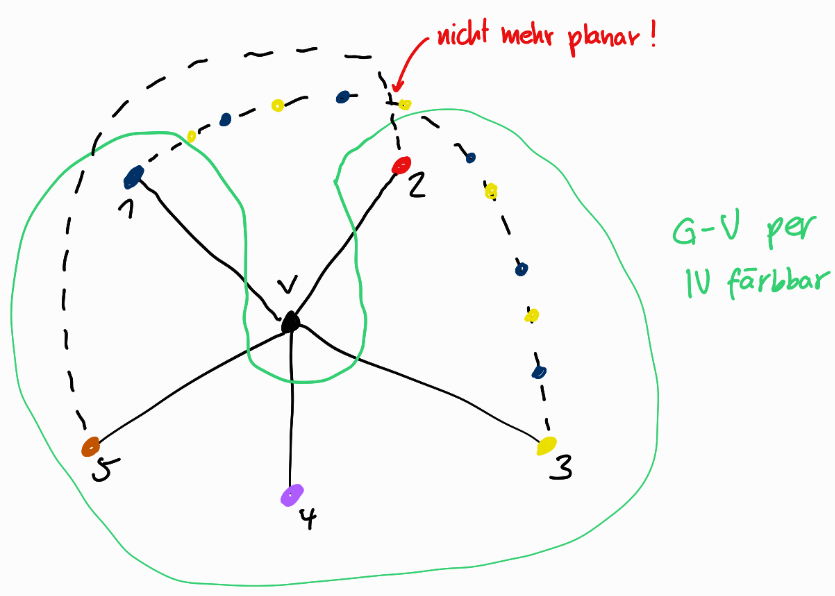
\includegraphics[width=0.4\textwidth]{images/5-f.png}
\end{center}

I.S.:
\begin{itemize}
	\item Nach Euler-Formel gibt es $v\in V$ mit $\text{deg}(v)\leq 5$
	\item Nach I.V. gibt es 5-Färbung von $G\setminus v$
	\item Betrachte Teilgraph, der nur blau-gelbe Knoten enthält:
	\begin{itemize}
		\item \underline{Fall 1}: 1 und 3 liegen in unterschiedlichen Zusammenhangskomponenten
		
		$\rightarrow$ Tausche in einer Zusammenhangskomponente alle blauen durch gelbe und alle gelben Knoten durch blaue aus $\rightarrow$ Farbe wird für $v$ frei
		\item \underline{Fall 2} (siehe Bild): 1 und 3 liegen in der selben Zusammenhangskomponente. Für rot-braun-Teilgraph können 2 und 5 nicht in der selben Zusammenhangskomponente liegen, da Graph sonst nicht mehr planar wäre
		
		$\rightarrow$ Farbe wird für $v$ frei
	\end{itemize}
\end{itemize}
\bigskip
\textbf{Definition}: Sei $G=(V,E)$ ein einfacher Graph. Sei $L\colon V\rightarrow 2^\N$ eine Listenzuweisung, d.h. $L(v)$ ist Menge von Zahlen / Farben. Eine \textbf{$\boldsymbol{L}$-Listenfärbung} von $G$ ist eine Knotenfärbung $c$ mit
\begin{itemize}
	\item $c(v)\in L(v)$ für jeden Knoten $v\in V$
	\item $c(u)\neq c(v)$ für jede Kante $uv\in E$
\end{itemize}
$G$ heißt \textbf{$\boldsymbol{k}$-listenfärbbar} wenn für jede Listenzuweisung $L$ mit $|L(v)|\geq k$ für jeden Knoten $v\in V$ eine $L$-Listenfärbung von $G$ existiert.
\begin{itemize}
	\item Kleinstes $k$, für das $G$ $k$-listenfärbbar ist, heißt \textbf{listenchromatische Zahl $\boldsymbol{\chi_{\text{list}}(G)}$}
\end{itemize}
\bigskip
\textbf{Beweisskizze zu Listenfärbungen}: 
\begin{itemize}
	\item $\chi_{\text{list}}(G)>k$: $\exists \text{ Listen } L\quad \nexists\text{ } L$-Listenfärbung 
	\item $\chi_{\text{list}}(G)\leq k$: $\forall \text{ Listen } L\quad \exists\text{ } L$-Listenfärbung
\end{itemize}
\bigskip
\textbf{Lemma}: Für jeden planaren Graphen gilt $\chi_{\text{list}}(G)\leq 6$

\textit{Beweis}: Die gleiche Argumentation wie für $\chi_{\text{planar}}\leq 6$ funktioniert\\

\textbf{Beobachtung}: Für jeden Graphen $G$ gilt $\chi_{\text{list}}(G)\geq \chi(G)$

\textit{Beweis}: 
\begin{itemize}
	\item Setze $L(v)=\{1,\ldots,k\}$ für jeden Knoten $v$
	\item Dann sind $L$-Listenfärbungen genau $k$-Knotenfärbungen $\implies \chi(G)\leq \chi_{\text{list}}(G)$
\end{itemize}
\bigskip
\textbf{Satz von Voigt}: Es gibt einen planaren Graphen mit $\chi_{\text{list}}(G)\geq 5$

\textit{Beweis}: Konstruiere einen planaren Graphen $G$ mit Listenzuweisung $L$, sodass 
\begin{itemize}
	\item $|L(v)|=4$ für jeden Knoten $v$
	\item keine $L$-Listenfärbung von $G$ existiert
\end{itemize}
Betrachte dazu folgendes Gadget $H(\alpha,\beta)$:
\begin{center}
	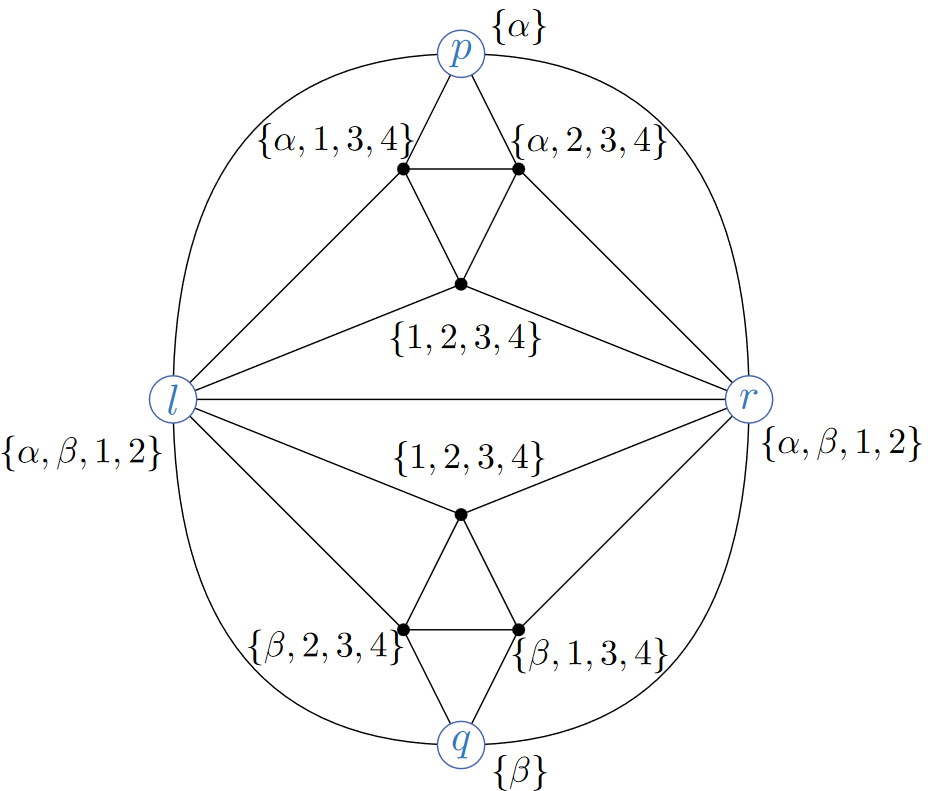
\includegraphics[width=0.45\textwidth]{images/lf-5.png}
\end{center}
Dieses Gadget ist nicht färbbar. Konstruiere nun aus 16 Gadgets den folgenden Graphen:
\begin{center}
	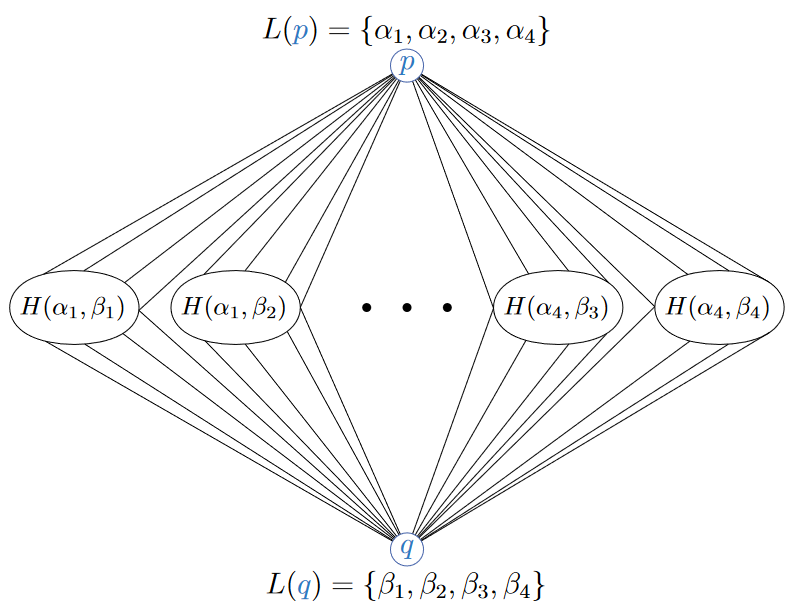
\includegraphics[width=0.5\textwidth]{images/lf-5-2.png}
\end{center}
Dieser ist nicht $L$-listenfärbbar, denn für jede Färbung $c$ ist Gadget $H(c(p),c(q))$ nicht färbbar.\\

\textbf{Weitere Sätze und Beobachtungen}:
\begin{itemize}
	\item Für jeden planaren Graphen gilt $\chi_{\text{list}}(G)\leq 5$ (\textbf{Satz von Thomassen})
	
	$\implies$ Mit obigem Satz folgt $\max\{\chi_{\text{list}}(G)\mid G \text{ planar}\}=5$
	\item Es gibt einen planaren Graphen mit $\chi(G)\geq 4$
	\item Für jeden planaren Graphen G gilt $\chi(G)\leq 4$ (\textbf{4-Farben-Satz})
	
	$\implies \chi_{\text{planar}}=4$ 
\end{itemize}
\bigskip
\textbf{Ziel}: Beweise $\chi_{\text{planar}}\leq 5$ mit einer stärkeren Aussage\\

\textbf{Satz}: Sei $G=(V,E)$ ein planarer Graph mit:
\begin{itemize}
	\item jede innere Facette ist ein Dreieck
	\item äußere Facette ist ein einfacher Kreis $C$
\end{itemize}
Seien $v_1,v_2$ zwei aufeinanderfolgende Knoten auf $C$ und $L$ eine Listenzuweisung mit:
\begin{itemize}
	\item $|L(v)|=5$ für $v\in V\setminus C$
	\item $|L(v)|=3$ für $v\in C\setminus \{v_1,v_2\}$
	\item $L(v_1)=\{\alpha\}, L(v_2)=\{\beta\}$ mit $\alpha\neq\beta$
\end{itemize}
Dann gibt es eine $L$-Listenfärbung von $G$.

\begin{wrapfigure}{r}{0.25\textwidth}
	\centering
	\vspace{-30pt}
	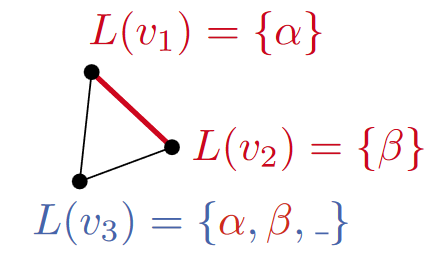
\includegraphics[width=0.25\textwidth]{images/thom-1.png}
	\vspace{40pt}
	\vspace{-120pt}
\end{wrapfigure}
\textit{Beweis}: Führe Induktion über $|V|$
\begin{itemize}
	\item I.A.: $|V|=3$. Wähle $c(v_3)\in L(v_3)\setminus\{\alpha,\beta\}$
	\item I.S.: $|V|\geq 4$. Betrachte nun 2 Fälle:
	\begin{itemize}
		\item \underline{Fall 1}: $C$ hat eine Sehne $e=v_iv_j$.
		Zerteile $G$ entlang $e$ in zwei Graphen $G_1,G_2$.
		O.B.d.A liegt $v_1v_2$ in $G_1$. 
		Nach IV gibt es eine Färbung $c_1$ von $G_1$.
		Sei $c_1(v_i)=\alpha'$ und $c_1(v_j)=\beta'$.
		Wende IV auf $G_2$ an mit Listen $\{\alpha'\}$ für $v_i$ und $\{\beta'\}$ für $v_j$. 
		$\rightarrow$ Färbung $c_2$ von $G_2$
		$\rightarrow$ Da $c_1$ und $c_2$ an der Sehne $v_iv_j$ übereinstimmen, erhalten wir eine Färbung von $G$.
		\begin{center}
			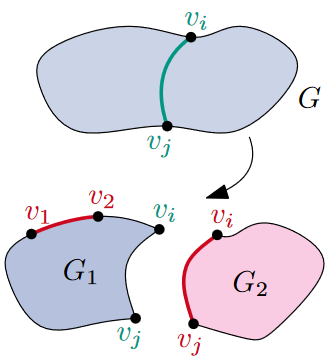
\includegraphics[width=0.25\textwidth]{images/thom-2.png}
		\end{center}
		\item \underline{Fall 2}: $C$ hat keine Sehne.
		Betrachte Nachbarn $v_p\neq v_2$ von $v_1$ auf C. Lösche $v_p$ auf $G$ und erhalte $G'$. $G'$ hat einfachen Kreis als äußere Facette, da $v_p$
		keine inzidente Sehne hat. Seien $\gamma_1,\gamma_2$ zwei Farben aus $L(v_p)\setminus\{\alpha\}$. Für jeden inneren Nachbarn $w$ von $v_p$ definiere $L'(w)=L(w)\setminus\{\gamma_1,\gamma_2\}$ und $L'(v)=L(v)$ für jeden anderen Knoten $v$. Nach IV gibt es $L'$-Listenfärbung von $G'$, sodass kein innerer Nachbar von $v_p$ die Farbe $\gamma_1$ oder $\gamma_2$ hat. Wähle $c(v_p)\in\{\gamma_1,\gamma_2\}\setminus c'(v_{p-1})$ und erhalte somit eine $L$-Listenfärbung $c$ von $G$.
	\end{itemize}
	\begin{center}
		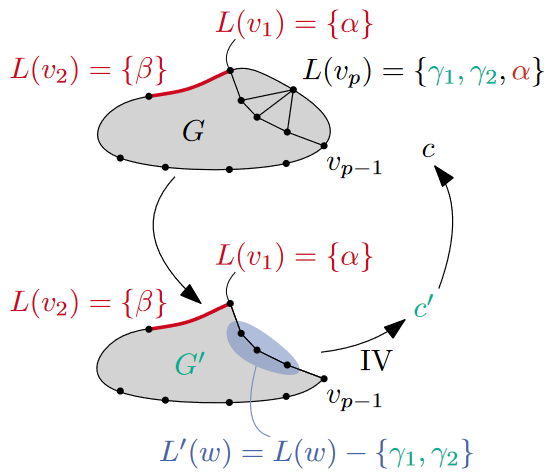
\includegraphics[width=0.35\textwidth]{images/thom-3.png}
	\end{center}
\end{itemize}

\textbf{Bemerkung}: Für jeden beliebigen planaren Graphen $G$ lassen sich Kanten und Knoten hinzufügen sowie Farben aus Listen entfernen, sodass der neue Graph $G'$ den Anforderungen des obigen Satzes entspricht. Damit wurde die Aussage $\chi(G)\leq\chi_{\text{list}(G)}\leq 5$ für jeden planaren Graphen $G$ bewiesen.

